\documentclass[%
thesis=student,% bachlor's or master's thesis
coverpage=false,% do not print an extra cover page
titlepage=false,% do not print an extra title page
headmarks=true, % headmarks can be switched on or off
german,% or `english`
font=libertine, % use `libertine` font; alternatives: `helvet` / `palatino` / `times`
math=newpxtx, % math font `newpxtx`; alternatives: `ams`, `pxtx`
BCOR=5mm,% binding correction - adapt accordingly
coverBCOR=11mm% binding correction for the cover - adapt accordingly
]{tumbook}

%
% --------------------------------------------------------------------------------
% Document Class
% --------------------------------------------------------------------------------
% We are using KOMA-Script
\documentclass[
    twoside,  % Default value already set????
    12pt,  % Font size 12pt
    numbers = noendperiod,  % Remove . in the header of a new chapter
    chapterprefix = true,
    bibliography = totoc,  % 
    % listof=totoc, % Adds "List of Figures / Tables" in the ToC
    DIV=calc
] {scrbook}

\usepackage[subpreambles=true]{standalone}
%% WARNING: Proceed with caution!

% -----------------------------------------------------------------------------------
% For package standalone
% -----------------------------------------------------------------------------------
\usepackage{import}

% -----------------------------------------------------------------------------------
% Language and typeset
% -----------------------------------------------------------------------------------
\usepackage[ngerman, english]{babel}

% Umlauts and other special characters (UTF-8)
% \usepackage[utf8]{inputenc}
\usepackage{fontspec}
\setsansfont{Arial}
% \usepackage[T1]{fontenc}  % Enable accented characters and umlauts
% LuaLatex doesn't need fontenc and uses UTF-8
% \usepackage{lmodern}  % Font face


% --------------------------------------------------------------------------------
% Page formatting
% --------------------------------------------------------------------------------
% Change the header/footer for chapter beginnings and normal pages
\usepackage[automark,headsepline]{scrlayer-scrpage}

% The package provides an easy and flexible user interface to customize the page
% layout, implementing auto-centering and auto-balancing mechanisms
% WARNING: WHEN CHANGING BCOR (Binding correction), the cover needs reworking!...
\newcommand{\theBCOR}{15mm}  % Define binding correction
\usepackage[
    bindingoffset=\theBCOR,
    % showframe, % Show boxes which indicate margins and paddings
    bottom = 3.5cm, % Margins
      left = 2.5cm,
     right = 2.5cm
] {geometry}

% The package 'float' provides a container for document objects which can not be
% broken over pages, such as tables and figures
% Needed for table and figure indexes  
\usepackage{float}

% support for landscape layout
\usepackage{lscape}

% support of \tablenotes command to add notes under table
\usepackage{threeparttable}

% To allow drawing more professional tables
\usepackage{booktabs}

% --------------------------------------------------------------------------------
% Contents
% --------------------------------------------------------------------------------
% Vector graphics (for Cover page)
\usepackage{tikz} 

% Allows additional parameters when including images
\usepackage{graphicx}

% Roman font family for all headings
\addtokomafont{disposition}{\rmfamily}

% Set the line spacing to 1.5
\usepackage[onehalfspacing]{setspace}

% Improves overall text spacing
% http://www.khirevich.com/latex/microtype/
\usepackage[stretch=10]{microtype}

% Math symbols like mu outside the math environment
\usepackage{textcomp}

% A comprehensive (SI) units package∗
% For defining SI units
\usepackage[
    range-units=single,         % Formatting ranges with single unit indication: 1 - 2 m
    range-phrase=-,             % Phrase for range: 1 - 2 m vs 1 to 2 m
    separate-uncertainty=true,  % sets +- between value and uncertainty 
    multi-part-units=repeat     % In expressions with multiple values (multi part numbers) 
                                % the unit is printed each time: 1 mm x 1 mm
] {siunitx}
% https://tex.stackexchange.com/questions/124488/multi-part-numbers-and-units-in-siunitx

% Allows Sourcecodes with highlighting 
\usepackage{listings}

% This package provides user control over the layout of the three basic list
% environments: enumerate, itemize and description
\usepackage{enumitem}
\setlist{nosep} % Remove the vertical space between \item elements in all lists

% ToDo Notes
% \setlength{\marginparwidth}{2cm}
\usepackage{todonotes}
\setuptodonotes{inline, inlinepar}
\reversemarginpar  % Put ToDo notes on the binding's side
% \usepackage{soul} % Colorful ToDo notes

% Check out colors here http://latexcolor.com/
\usepackage{xcolor}

\usepackage{amsmath}    % alignment of equations

% --------------------------------------------------------------------------------
% Other elements
% --------------------------------------------------------------------------------
% Blindtext: Organic looking text dummy
\usepackage{blindtext}

% Hyperlinks within the document (PDF)
% "hidelinks" hides visual highlighting of links
\usepackage[hidelinks]{hyperref}

% Package for Glossary and Index (Acronyms are listed in a separate list) 
\usepackage[acronym, nogroupskip]{glossaries} % groupskip: alphabetic grouping of entries

\usepackage{xltabular}   % <------- FOR glossaries

% Integration and management of bibliographies
\usepackage{csquotes}   % backend=biber in biblatex needs this package
\usepackage[
    style=ieee,   % style of the bibliography, entries are sorted in alphabetic order. "ieee" is another common style.
    backend=biber,      % based on package 'biber' 
    bibencoding=ascii   % ASCII Text encoding; may use "utf8" instead
] {biblatex}

% --------------------------------------------------------------------------------
%                               PATHS & FILES
% --------------------------------------------------------------------------------
% Fix paths for standalone compiling
\ifstandalone
    \def \home {..}
\else
    \def \home {.}
\fi

% Package: scrlayer-scrpage
% \def \stylePath {\home/settings+/style/page}
\input{\home/settings+/style/page}  % Load page style

% Package: graphicx
\graphicspath{{\home/images/}}  % Set path to images

% Package: listings
\input{\home/settings+/style/code.tex}  % Set path to style file
\lstset{inputpath={\home/code/}} % Default path to code listings

% Package: glossaries
\input{\home/settings+/style/symbols}  % Set path to symbols list style file
\input{\home/settings+/style/acronyms}  % Set path to acronym list style file
\input{\home/references/glossary_acronyms}  % Load glossary, symbol and acronyms list

% Package: biblatex
\addbibresource{\home/references/references.bib}  % Set path to bib resources

% Custom variables
\makeatletter
% ----------------------------------------------------------------------------
% Custom Colors (RGB 0-255, rgb 0-1)
% ----------------------------------------------------------------------------
\definecolor{dartmouthgreen}{rgb}{0.05, 0.5, 0.06}
\definecolor{myBlueFaded}{RGB}{80, 127, 186}
\definecolor{myBlue}{RGB}{42, 93, 156}

% Colors for code listings
\definecolor{darkgreen}{RGB}{0,100,0}
\definecolor{steelblue}{rgb}{0.27, 0.51, 0.71}

% ----------------------------------------------------------------------------
% Shorthands for custom colors and trademarks
% ----------------------------------------------------------------------------
\newcommand\red[1]{\textcolor{red}{\textbf{#1}}}
\newcommand\green[1]{\textcolor{dartmouthgreen}{#1}}
\newcommand\blue[1]{\textcolor{blue}{#1}}
\newcommand{\orange}[1]{{\color{orange}#1}}

% Quick access to business symbols via \TReg, \TCop and \TTra
\def\TReg{\textsuperscript{\tiny{\textregistered}}}
\def\TCop{\textsuperscript{\textcopyright}}
\def\TTra{\textsuperscript{\texttrademark}}

% ----------------------------------------------------------------------------
% Defining variables for cover pages and declaration of independence
% ----------------------------------------------------------------------------
% Author
\newcommand*{\matrikelnr}[1]{\gdef\@matrikelnr{#1}}

% University
\newcommand*{\uniEn}{University of Freiburg}
\newcommand*{\uni}{Albert-Ludwigs-Universität Freiburg}
\newcommand*{\institute}[1]{\gdef\@institute{#1}}
\newcommand*{\chair}[1]{\gdef\@chair{#1}}

% Thesis
\newcommand*{\thesisType}[1]{\gdef\@thesisType{#1}}
\newcommand*{\thesisTitle}[1]{\gdef\@thesisTitle{#1}}
\newcommand*{\submitDate}[1]{\gdef\@submitDate{#1}}
\newcommand*{\editingTime}[1]{\gdef\@editingTime{#1}}

% Examiners
\newcommand*{\firstExaminer}[1]{\gdef\@firstExaminer{#1}}
\newcommand*{\firstExaminerDepartment}[1]{\gdef\@firstExaminerDepartment{#1}}
\newcommand*{\firstExaminerChair}[1]{\gdef\@firstExaminerChair{#1}}
\newcommand*{\secondExaminer}[1]{\gdef\@secondExaminer{#1}}
\newcommand*{\secondExaminerDepartment}[1]{\gdef\@secondExaminerDepartment{#1}}
\newcommand*{\secondExaminerChair}[1]{\gdef\@secondExaminerChair{#1}}

% Supervisor
\newcommand*{\supervisor}[1]{\gdef\@supervisor{#1}}
\newcommand*{\supervisorDepartment}[1]{\gdef\@supervisorDepartment{#1}}
\newcommand*{\supervisorChair}[1]{\gdef\@supervisorChair{#1}}

% ----------------------------------------------------------------------------
% ToDo notes
% ----------------------------------------------------------------------------
% Let's fix up the ugly spacing of the 'todonotes' package
\renewcommand{\todo}[2][inline]{%
    \vspace{2mm}
    \@todo[#1]{#2}
    \vspace{-1mm}
}
\makeatother

% --------------------------------------------------------------------------------
%                                   OPTIONAL
% --------------------------------------------------------------------------------


% Simple arithmetic for LaTeX commands
% \usepackage{calc}

% Document Elements
% -------------------

% Index
% \usepackage{imakeidx}

% compact Lists
%\usepackage{paralist}

% visual improvements for citations
% \usepackage{epigraph}

% Create pseudo code
% https://www.overleaf.com/learn/latex/Algorithms
% \usepackage{algorithm}
% \usepackage{algorithmic}
%\usepackage[noend]{algpseudocode}

% Formatting
% -------------------
% Tweaks for scrbook, redefines commands of other packages
% \usepackage{scrhack}

% Intelligent space separator (nice for superscript?)
% \usepackage{xspace}

% Allows breaks within tables
%\usepackage{tabularx}

% Allows for page breaks in tables
% \usepackage{longtable}

% allows modifying of captions
% \usepackage{caption}

% Multiline comments
%\usepackage{verbatim}

% % Custom colors
% \definecolor{dartmouthgreen}{rgb}{0.05, 0.5, 0.06}

% IF you want to define unicode characters
% \DeclareUnicodeCharacter{0229}{\c{e}}
% \DeclareUnicodeCharacter{0306}{\u{Z}}


% Document elements
% ------------------------------------

% Table package
% \usepackage{booktabs}

% Pie diagram
% \usepackage{datapie}

% Side by Side images
% \usepackage{subcaption}

% For landscape tables
%\usepackage{pdflscape}
%\usepackage{afterpage}

% Graphics can be flow around by text
%\usepackage{wrapfig}

\usepackage{tikz}
\usetikzlibrary{arrows.meta, positioning, calc, automata, shapes.geometric}
\usepackage{pgfplots}
%\makeatletter %redefine some labels from the TUM template
%\provideName{\@tum@examiner@}{Supervisor}{Themensteller} % or `Themenstellerin`
%\provideName{\@tum@supervisor@}{Advisors}{Betreuer} % or `Advisor` / `Betreuerin`
\makeatother

\usepackage{booktabs}% for more beautiful tables
\usepackage{cleveref}% intelligent references
\usepackage{eso-pic}
\usepackage{diffcoeff}
\usepackage{amsmath}
\usepackage{amsthm}
\newtheoremstyle{break}
{\topsep}   % Platz oberhalb
{\topsep}   % Platz unterhalb
{\itshape}  % Schriftart im Textkörper
{0pt}       % Einzug (keiner)
{\bfseries} % Schriftart im Kopf
{.}         % Punkt nach Theorem-Name
{\newline}  % Zeilenabstand nach Theorem-Name
{}          % Zusätzliche Spezifikation


\theoremstyle{break}
\newtheorem{definition}{Definition}[section]
\newtheorem{theorem}[definition]{Satz}

%Literatur
\usepackage[%
    backend=bibtex, %, or `biber` on more up-to-date systems
    sortcites, % sort automatically
    sorting=nty, % sort order
    safeinputenc, % solves problems with unicode-formatted author names etc.
    citestyle=alphabetic, %
    bibstyle=alphabetic, %
    hyperref=true, % provide clickable links
    maxbibnames=3, % shorten author list for more than 3 names
    maxcitenames=3, % use at most 3 names for key
    url=false, % do not print URLs
    doi=false, % do not print DOIs
    giveninits=true,
    ]%
{biblatex}
\addbibresource{literature.bib}

% automatische Anführungszeichen
\usepackage[autostyle=true]{csquotes}


\title{Verzerrung der Inferenz bei der Verwendung gemischter Modelle in latenten Repräsentationen}


\author{Yannick Bantel}

\degree{Bachelor of Science}% or `Bachlor of Science`
\dateSubmitted{23. Juli 202}% preferably use some universally recognized date format

\examiner{Prof.\@ Dr.\@ Harald Binder}% `Themensteller`
\supervisor{Clemens Schächter}% `Betreuer`

% Title Page
\title{Titel der Bachelorarbeit}
\author{Dein Name}
\date{Abgabedatum}

% Command to include background image
\newcommand\BackgroundPic{
	\put(0,0){
		\parbox[b][\paperheight]{\paperwidth}{
			\vfill
			\centering
			
\includegraphics[width=\paperwidth,height=\paperheight,keepaspectratio]{deckblatt.pdf}
			\vfill
}}}

% Command to include logo image
\newcommand\LogoPic{
	\put(\LenToUnit{0.7\paperwidth},\LenToUnit{0.75\paperheight}){
		\parbox[b][\paperheight]{\paperwidth}{
			\vfill
			\raggedleft
			
\includegraphics[width=0.4\textwidth]{Logo_Uni_alt.pdf}
			\vfill
}}}

\begin{document}
	% Title Page
\begin{titlepage}
	\AddToShipoutPicture*{\BackgroundPic}
	\AddToShipoutPicture*{\LogoPic}
	\centering
	\vspace*{1cm}
	
	\vfill
	
	\textsc{\LARGE Albert-Ludwigs-Universität Freiburg}\\[1.5cm]
	
	\textsc{\Large Bachelorarbeit}\\[0.5cm]
	
	\rule{\linewidth}{0.5mm} \\[0.4cm]
	{ \huge \bfseries Verzerrung der Inferenz bei Verwendung gemischter Modelle in latenten Repräsentationen}\\[0.4cm]
	\rule{\linewidth}{0.5mm} \\[1.5cm]
	
	\begin{minipage}{0.4\textwidth}
		\begin{flushleft} \large
			\emph{Autor:}\\
			Yannick Bantel \\
			\vspace{5pt}
			\emph{Professor:} \\
			Prof. Dr. Harald Binder \\
			\vspace{5pt}
			\emph{Betreuer:} \\
			Clemens Schächter\\

		\end{flushleft}
	\end{minipage}
	\begin{minipage}{0.4\textwidth}
		\begin{flushright} \large
			\emph{Abgabedatum:} \\
			\today
		\end{flushright}
	\end{minipage}\\[3cm]
	
	\begin{tikzpicture}[remember picture, overlay]
		\node[anchor=south east, xshift=-2cm, yshift=3cm] at (current page.south east) {
			
\includegraphics[width=0.2\textwidth]{Logo_Uni_alt.pdf}
		};
	\end{tikzpicture}
	
	\vfill
	

	
\end{titlepage}
%\frontmatter
%\maketitle
\section*{Zusammenfassung}
Eine kurze Zusammenfassung der Arbeit auf Deutsch.

\section*{Abstract}
A brief abstract of this thesis in English.

\cleardoublepage{}

\tableofcontents

\mainmatter{}

%%---------------EINLEITUNG--------------------------------------------------
\chapter{Einleitung}

In der modernen Datenanalyse spielen gemischte Modelle eine zentrale Rolle, da sie es ermöglichen, sowohl feste als auch zufällige Effekte zu berücksichtigen. Dies macht sie besonders in den Bereichen der Biostatistik, der Sozialwissenschaften und der ökonomischen Modellierung populär.\\ 
Im Rahmen dieser Arbeit werden gemischte Modelle auf die Analyse medizinischer Daten angewendet. Mit dem Aufkommen von Big Data und komplexen Datenstrukturen hat sich der Fokus zunehmend auf die effiziente und genaue Extraktion von Informationen aus großen und oft unübersichtlichen Datensätzen verlagert.\\ 
In diesem Zusammenhang gewinnen latente Repräsentationen an Bedeutung, da sie es ermöglichen, inhärente Strukturen innerhalb der Daten zu identifizieren und zu nutzen, um tiefere Einblicke zu gewinnen.\\
\\
Die Integration von gemischten Modellen in latente Repräsentationen birgt jedoch das Risiko einer Verzerrung der Inferenzergebnisse, was die Genauigkeit und Zuverlässigkeit der aus den Daten gezogenen Schlussfolgerungen erheblich beeinträchtigen kann.\\ 
Die vorliegende Arbeit widmet sich der Untersuchung von Verzerrungen, die bei der Anwendung gemischter Modelle auf latente Repräsentationen auftreten können. Das Ziel dieser Arbeit ist es, die Mechanismen zu verstehen, die zu diesen Verzerrungen führen, sowie Methoden zu entwickeln, um ihre Auswirkungen zu minimieren.\\
\\
Das Problem der Verzerrung ist von besonderer Relevanz, da eine fehlerhafte Inferenz zu Fehlentscheidungen führen kann, die in praktischen Anwendungen schwerwiegende Konsequenzen haben können.\\
Die Arbeit zielt darauf ab, durch eine sorgfältige Analyse und Bewertung von gemischten Modellansätzen in Verbindung mit latenten Repräsentationen einen Beitrag zur Verbesserung der Modellgenauigkeit und der Zuverlässigkeit von Inferenzschlüssen zu leisten.\\
\\
Die Arbeit ist in mehrere Teile gegliedert, die zunächst die theoretischen Grundlagen von gemischten Modellen und latenten Repräsentationen behandeln. Im Anschluss erfolgt eine Diskussion der Methoden zur Messung und Korrektur von Verzerrungen. \\
Im Anschluss werden die zuvor theoretisch erörterten Konzepte anhand von empirischen Studien praktisch angewendet und evaluiert. Auf Basis der gewonnenen Erkenntnisse werden abschließend Empfehlungen für die Anwendung dieser Techniken in Forschung und Praxis gegeben.\\
\\
\subsection{Motivation}


%%-------------THEORETISCHE-GRUNDLAGEN---------------------------------------
\chapter{Theoretische Grundlagen}
Im Vorfeld der Erörterung der Methodik dieser Arbeit ist eine theoretische Aufarbeitung der behandelten Themen unabdingbar. In diesem Kapitel erfolgt eine ausführliche Beschreibung und Behandlung der theoretischen Aspekte dieser Arbeit. Es werden sowohl lineare gemischte Modelle als auch die Theorie hinter Variational Autoencodern eingeführt und beschrieben. Im Folgenden wird insbesondere auf die für die Analyse der Modelle notwendige Theorie eingegangen, wie beispielsweise die Likelihood-Berechnung und der Likelihood-Ratio-Test.

%----------------------------------------------------------------------------

%-----------------------VARIATIONAL-AUTOENCODER------------------------------

%----------------------------------------------------------------------------
\section{Variational Autoencoder (VAE)}
Die Anwendung der gemischten Modelle auf einer latenten Repräsentation erfolgt mittels Variational Auto-Encoder (VAE). Variational Auto-Encoder sind generative Modelle, welche versuchen die zugrunde liegende Struktur der Inputdaten x im latenten Raum zu modellieren. Im Vergleich zu normalen Autoencoder, welche den latenten Raum durch feste Punkte modellieren, wie es in Abbildung \ref{fig:vae1} dargestellt ist, wird der latente Raum in der Erweiterung VAE durch eine Wahrscheinlichkeitsverteilung (Normalverteilung) modelliert.
\begin{figure}
	\centering
	\begin{tikzpicture}[auto, thick, node distance=2cm, >=stealth]
		
		% Define styles
		\tikzstyle{latent} = [rectangle, draw, fill=blue!20, text centered, minimum width=1cm, minimum height=2cm]
		\tikzstyle{input} = [rectangle, draw, fill=yellow!20,text centered, minimum width=1cm, minimum height=3cm]
		\tikzstyle{output} = [rectangle,draw, fill=yellow!20, text centered, minimum width=1cm, minimum height=3cm]
		
		% Nodes
		\node[input, name=input] (input) {x};
		\node[latent, right of=input, node distance=6cm, minimum width=1cm, minimum height=2cm] (z) {$Z$};
		\node[output, right of=z, node distance=6cm] (output) {$\hat{x}$};
		
		% Custom trapezoids for encoder and decoder
		\draw[fill=gray!20] (3,2) -- (3,-2) -- (5,-1) -- (5,1) -- cycle;
		\node at (3.75, 0) {Encoder};
		
		\draw[fill=green!20] (7,1) -- (7,-1) -- (9,-2) -- (9,2) -- cycle;
		\node at (8, 0) {Decoder};
		
		% Arrows
		\draw[->] (input.east) -- (2.75,0);
		\draw[->] (5,0) -- (z.west);
		\draw[->] (z.east) -- (7,0);
		\draw[->] (9.75,0) -- (output.west);
		
		% Labels
		\node[above of=input, node distance=2cm] {Input};
		\node[above of=z, node distance=1.5cm] {Latent Space};
		\node[above of=output, node distance=2cm] {Reconstructed Data};
		
		% Additional Text
		\draw[->, thick] (output.south) |- ++(0, -2.5cm) -| (input.south);
		\node[below of=z, node distance=3.5cm, text width=6cm, align=center] {Reconstruction Loss};
		
		
	\end{tikzpicture}
	\caption{Aufbau eines herkömmlichen Autoencoders}
	\label{fig:autoencoder}
\end{figure}
\subsection{Strucktur des VAEs}
Die Architektur eines VAE basiert auf zwei neuronalen Netzwerken: einem Encoder, der die Inputdaten x im latenten Raum als Verteilung kodiert, und einem Decoder, der aus den latenten Daten versucht die Originaldaten zu rekonstruieren. Diese Module lernen die wesentlichen Merkmale der Eingabedaten zu extrahieren und eine komprimierte Version dieser Daten zu erzeugen.\\
\\
\begin{figure}
	\centering
	
	\begin{tikzpicture}[auto, thick, node distance=2cm, >=stealth]
		
		% Define block styles
		\tikzstyle{block} = [trapezium, trapezium left angle=70, trapezium right angle=110, minimum height=3cm, draw, fill=gray!20, text centered]
		\tikzstyle{block2} = [trapezium, trapezium left angle=110, trapezium right angle=70, minimum height=3cm, draw, fill=green!20, text centered]
		\tikzstyle{square} = [rectangle, draw, fill=red!20, minimum size=1.5cm, text centered]
		\tikzstyle{latent} = [rectangle, draw, fill=blue!20, minimum size=1.5cm, text centered]
		
		% Nodes		
		\node[rectangle, draw, fill=yellow!20, minimum height=3cm, minimum width=1cm, text centered] (input) {$\mathbf{x}$};
		\draw[fill=gray!20] (1,2) -- (1,-2) -- (3,-1) -- (3,1) -- cycle;
		\node[right of=input, node distance=2cm] (encoder) {$q_{\phi}(z \mid x)$};
		\node[square, right of=encoder, node distance=2.5cm] (mu) {$\mu$};
		\node[square, below of=mu, node distance=2cm] (sigma) {$\sigma$};
		\node[latent, right of=mu, node distance=2cm] (z) {$\mathbf{Z}$};
		\draw[fill=green!20] (8,1) -- (8,-1) -- (10,-2) -- (10,2) -- cycle;
		\node[right of=z, node distance=2.5cm] (decoder) { $p_{\theta}(x \mid z)$};	
		\node[rectangle, draw, fill=yellow!20, minimum height=3cm, minimum width=1cm, text centered, right of=decoder, node distance=3cm] (output) {$\hat{\mathbf{x}}$};
		
		
		
		% Arrows
		\draw[->] (input) -- (1,0);
		\draw[->] (3,0) -- (mu);
		\draw[->] (3,0) -- (sigma);
		\draw[->] (mu) -- (z);
		\draw[->] (sigma) -- (z);
		\draw[->] (z) -- (8,0);
		\draw[->] (10,0) -- (output);
		
		% Labels
		\node[above of=input, node distance=1.75cm] {Input Data};
		\node[above of=encoder, node distance=0.8cm] {Encoder};
		\node[above of=z, node distance=1cm] {Latent Space};
		\node[above of=decoder, node distance=0.8cm] {Decoder};
		\node[above of=output, node distance=1.75cm] {Reconstructed Data};
		
		\node[below of=sigma, node distance=1.2cm] {Standard Deviation};
		
		% Additional Text
		\draw[->, thick] (input.south) |- ++(0, -2.5cm) -| (output.south);
		\node[below of=encoder, node distance=4.5cm, text width=6cm, align=center] {Reconstruction Loss + KL Divergence};
		
	\end{tikzpicture}
	\caption{Darstellung der Architektur eines Variational Autoencoders (VAE)}
	\label{fig:vae}
\end{figure}
VAEs sind für die Modellierung latenter Repräsentationen von großem Interesse, da sie hochdimensionale Datensätze mit Hilfe des Encoders im latenten Raum niedrigdimensional darstellen können. Dies reduziert die Komplexität der Modellierung und ermöglicht es, gemischte Modelle effizienter und genauer zu betreiben. Im Gegensatz zu herkömmlichen Autoencodern ist der VAE in der Lage, nicht nur den Eingabedatensatz zu rekonstruieren, sondern auch neue Inhalte zu generieren. Dies wird durch die verbesserte Repräsentation ermöglicht(vgl. \cite{bigdata-insider-vae}).\\
\\
\textbf{Latenter Raum}\\
Variablen, die man nicht direkt messen kann, demnach nicht Teil des erhaltenen Datensatzes sind, bezeichnet man als latente Variablen. Sie werden erst mithilfe der gegebenen Daten erschlossen und ergeben im Verbund den latenten Raum.\\
Im VAE werden die latenten Variablen z aus der priori-Verteilung $p_\theta(x)$ gezogen, welche eine multivariate Normalverteilung $p_\theta(x) = \mathcal{N}(z;0,I) $ ist. Die latenten Daten werden aus den Inputdaten durch den Encoder  gezogen, welcher die posteriori Verteilung durch eine variable Verteilung $q_\phi(z,x)$ approximiert. Der Encoder erlernt somit zwei Vektoren, nämlich den Mittelwert \( \mu \) und die Standardabweichung \( \sigma^2 \) der Normalverteilung $q_\phi(z,x) = \mathcal{N}(z;\mu(x),\sigma^2(x))$.\\
Der Decoder versucht aus den latenten Variablen die Inputdaten x durch die likelihood-Verteilung $p_\theta(x|z)$  zu rekonstruieren. Die  Wahrscheinlichkeit, dass die beobachteten Daten aus den latenten Repräsentationen generiert wurden, wird durch dieses Modell modelliert. Auch hier wird typischerweise eine Normalverteilung angenommen, sofern die  Daten reellwertig sind. Im Falle binärer Daten wird die Verteilung als Bernoulli-Verteilung modelliert. \\ Für weiterführende Details wird auf die Publikation \cite{Auto-EncodingVariationalBayes} verwiesen.\\
\subsection{Training VAE}
Ein VAE stellt ein spezifisches Beispiel einer Variational Inference (VI) dar. Die Zielsetzung einer VI besteht in der Berechnung der  Posteriori-Verteilung $p(z|x)$ der latenten Variablen in Abhängigkeit von den Input-Daten.  Die Berechnung dieser Verteilung ist besonders bei komplexen Modellen mit Schwierigkeiten verbunden. Infolgedessen approximiert der VAE die Posteriori-Verteilung durch eine einfachere Verteilung $q_\phi(x)$. Das Ziel von VIs besteht folglich in der Minimierung des Rekonstruktionsfehlers sowie der Kullback-Leibler-Divergenz zwischen der tatsächlichen Posteriori-Verteilung $p(z|x)$ und  der approximierten verteilung $q_\phi(x)$. 
\begin{definition}[Kullback-Leibler-Divergenz (KL-Divergenz)]
Sei $q_\phi(z|x)$ die approximierte Posteriori-Gauß-Verteilung und $p(z)$ die Priori-Gauß-Verteilung. Dann ist die KL-Divergenz definiert als
$$D_{KL}(q_\phi(z|x)||p(z))= \int q_\phi(z|x) \log \left(\frac{q_\phi(z|x)}{p(z)} \right)dz$$
\end{definition}\noindent
Da die Berechnung von  $p(z)$ mit Schwierigkeiten verbunden ist, wird  stattdessen die Evidence Lower Bound (ELBO) durch Stochastic Gradient Descent (SGD) oder andere ähnliche Verfahren optimiert.\\
Das Objekt der Optimierung im VAE ist somit der ELBO. \\
Im Folgenden wird die log-Likelihood der Daten betrachtet, um den ELBO herzuleiten (vgl. \cite{IntroductiontoVAEs}).\\
\begin{align}
 	\log p_\theta(x) &= \log p_\theta(x) * \overbrace{\int q_\phi(z|x) dz}^{=1} \\
 	&= \int \log p_\theta(x) q_\phi(z|x) dz \\
 	&= \mathbb{E}_{q_\phi(z|x)}[\log p_\theta(x)] \\
 	&= \mathbb{E}_{q_\phi(z|x)}\left[\log\left[ \frac{p_\theta(x,z)}{p_\theta(z|x)}\right]\right] \\
 	&= \mathbb{E}_{q_\phi(z|x)}\left[\log\left[ \frac{p_\theta(x,z)q_\phi(z|x)}{q_\phi(z|x)p_\theta(z|x)}\right]\right] \\
 	&= \underbrace{\mathbb{E}_{q_\phi(z|x)}\left[\log\left[ \frac{p_\theta(x,z)}{q_\phi(z|x)}\right]\right]}_{\substack{\text{$= \mathcal{L}_{\theta,\phi}(x)$}\\\text{(ELBO)}}} + \underbrace{\mathbb{E}_{q_\phi(z|x)}\left[\log\left[ \frac{q_\phi(z|x)}{p_\theta(z|x)}\right]\right]}_{=D_{KL}(q_\phi(z|x)||p_\theta(z|x))} \label{ELBO & DKL Gleichung}
\end{align}
Der zweite Term in der Gleichung ist die nicht negative Kullback-Leibler-Divergenz (KL-Divergenz) zwischen $q_\phi(z|x)$ und $p_\theta(z|x))$. Der erste Term in Gleichung \ref{ELBO & DKL Gleichung} stellt den Evidence-Lower-Bound, kurz ELBO, dar: 
\begin{definition}[Evidence Lower Bound (ELBO) für VAEs]
	Sei $q_\phi(z|x)$ das Encoder Modell und $p_\theta(x,z)$ das Decoder Modell. Der ELBO ist definiert durch
	$$ \mathcal{L}_{\theta,\phi}(x) = \mathbb{E}_{q_\phi(z|x)}[\log p_\theta(x,z) - \log q_\phi(z|x)] $$ 
\end{definition}\noindent
Die Umstellung der Gleichung \ref{ELBO & DKL Gleichung} zeigt, dass der ELBO eine untere Schranke für die log-likelihood der Daten darstellt, da die KL-Divergenz nicht negativ ist: 
\begin{align}
	\mathcal{L}_{\theta,\phi}(x) &= \log p_\theta(x) - D_{KL}(q_\phi(z|x)||p_\theta(z|x)) \\
	&\leq 	\log p_\theta(x) 
\end{align}\noindent
Die Gleichung kann alternativ mit der Jensenschen Ungleichung (vgl. \cite{JensenscheUngleichung}) wie folgt umgestellt werden:
\begin{align}
	\log p_\theta(x) &= \log \int p_\theta(x,z) dz \\
	&= \log \int p_\theta(x,z) \frac{q_\phi(z|x)}{q_\phi(z|x)} dz \\
	& = \log \mathbb{E}_{q_\phi(z|x)}\left[\frac{p_\theta(x,z)}{q_\phi(z|x)}\right] \\
	& \overset{Jensen}{\geq} \mathbb{E}_{q_\phi(z|x)}\left[\log \frac{p_\theta(x,z)}{q_\phi(z|x)}\right] = \mathcal{L}_{\theta,\phi}(x)
\end{align}\noindent
Es ist sofort ersichtlich, dass die log-likelihood $p_\theta(x)$ durch Maximieren der ELBO bzgl. $\theta$ und  $\phi$ selbst maximiert wird.
Folglich verbessert sich die Qualität unseres generatives Modells. Gleichzeitig wird  dadurch die KL-Divergenz der Approximation $q_\phi(z|x)$ an den wahren Posteriori $p_\theta(z|x)$ minimiert. Daher wird die Approximation $q_\phi(z|x)$ optimiert. 
Die ELBO kann durch stochastische Gradientenverfahren optimiert werden.\\
\\
Die Berechnung des Gradienten von $\mathcal{L}_{\theta,\phi}(x) = \mathbb{E}_{q_\phi(z|x)}\left[\log p_\theta(x,z)- \log q_\phi(z|x)\right]$ bezüglich $\theta$ kann problematisch sein. Der Monte-Carlo-Schätzer für Gradienten ist eine gängige Methode und kann wie folgt definiert werden (vgl. \cite{MonteCarloEstimation}): 
\begin{align}
 \nabla_\phi \mathbb{E}_{q_\phi(z)}[f(z)]= \mathbb{E}_{q_\phi(z)}[f(z)\nabla_{q_\phi(z)}\log q_\phi(z)] \approx \frac{1}{L} \sum_{l=1}^{L}f(z)\nabla_{q_\phi(z^{(l)})}\log q_\phi(z^{(l)}) \label{MonteCarloEstimator}
\end{align}
wobei $z^{(l)} \sim q_\phi(z|x^{(i)})$ ist. 
In der Regel stellt dies keine Herausforderung dar. Allerdings ist $q_\phi(z|x)$ nun auch abhängig von  $\phi$, sodass der Monte Carlo Gradienten-Schätzer nicht direkt berechnet werden kann. \\
Zur Lösung dieses Problems wird der sogenannte Reparameterization-Trick eingesetzt, welcher die Zufallsvariable transformiert um die Gradienten-Berechnung zu vereinfachen.  
\subsubsection{Reparametrisierungs Trick}
Der Reparameterisierungs-Trick ist eine Methode zur Vereinfachung der Gradientenberechnung in Variational-Autoencodern. Er ermöglicht eine effizientere Berechnung der Gradienten der Evidence Lower Bound und somit eine effizientere Optimierung der ELBO. Der Reparameterization Trick transformiert die Zufallsvariable z in eine deterministische Funktion von einer Hilfsvariablen $\epsilon$, was es erleichtert Backpropagation durchzuführen.
Sei also die latente Variable z, die aus $q_\phi(z|x)$ gezogen wurde, gegeben. Die latente Variable z wird nun als deterministische Funktion einer Hilfsvariablen $\epsilon$, unabhängig von x und $\phi$, ausgedrückt. 
Die Transformation sieht dann wie folgt aus
$$ z = g_\phi(\epsilon, x)$$
$g_\phi(\epsilon,x) $ ist dabei eine differenzierbare Funktion und $\epsilon$ eine Zufallsvariable mit einer bekannten Verteilung (z.B. $\epsilon \sim \mathcal{N}(0,I)$).\\
Im Falle einer Gaußverteilung $z \sim \mathcal{N}(\mu, \sigma^2)$ könnte die Umparametrisierung wie folgt aussehen 
$$z=\mu + \sigma \odot \epsilon \hspace{10pt}\text{mit} \hspace{2pt} \epsilon\sim N(0,I).$$ Dies ist in  Abbildung \ref{fig:vae_reparameterization_trick} veranschaulicht.
Dadurch können die Gradienten bezüglich $\mu$ und $\sigma$ effizient berechnet werden, da der Erwartungswert über $q_\phi(z|x)$ sich nun als Erwartungswert über $\epsilon$ schreiben lässt.
\\
Wir können den Trick direkt auf Gleichung \ref{MonteCarloEstimator} anwenden (vgl. \cite{MonteCarloEstimation}). Es gilt
\begin{align}
	 \nabla_\phi \mathbb{E}_{q_\phi(z)}[f(z)] &= \nabla_\phi \int q_\phi(z) f(z) dz \\
	 &= \nabla_\phi \int q_\epsilon(z) f(g_\phi(\epsilon;\phi)) d\epsilon \\
	 &= \nabla_\phi \mathbb{E}_{q(\epsilon)}[g_\phi(\epsilon,z)]
\end{align}
\begin{figure}
	\centering
	\begin{tikzpicture}[auto, thick, node distance=2cm, >=stealth]
		
		% Define block styles
		\tikzstyle{block} = [trapezium, trapezium left angle=70, trapezium right angle=110, minimum height=3cm, draw, fill=gray!20, text centered]
		\tikzstyle{block2} = [trapezium, trapezium left angle=110, trapezium right angle=70, minimum height=3cm, draw, fill=green!20, text centered]
		\tikzstyle{square} = [rectangle, draw, fill=red!20, minimum size=1.5cm, text centered]
		\tikzstyle{latent} = [rectangle, draw, fill=blue!20, minimum size=1.5cm, text centered]
		
		% Nodes		
		\node[rectangle, draw, fill=yellow!20, minimum height=3cm, minimum width=1cm, text centered] (input) {$\mathbf{x}$};
		\draw[fill=gray!20] (1,2) -- (1,-2) -- (3,-1) -- (3,1) -- cycle;
		\node[right of=input, node distance=2cm] (encoder) {$q_{\phi}(z \mid x)$};
		\node[square, right of=encoder, node distance=2.5cm] (mu) {$\mu$};
		\node[square, below of=mu, node distance=2cm] (sigma) {$\sigma$};
		\node[latent, right of=mu, node distance=2cm] (z) {$\mathbf{z = \mu + \sigma \odot \epsilon}$};
		\node[square, above of=mu, node distance=2cm] (epsilon) {$\epsilon$};
		\draw[fill=green!20] (8,1) -- (8,-1) -- (10,-2) -- (10,2) -- cycle;
		\node[right of=z, node distance=2.5cm] (decoder) { $p_{\theta}(x \mid z)$};	
		\node[rectangle, draw, fill=yellow!20, minimum height=3cm, minimum width=1cm, text centered, right of=decoder, node distance=3cm] (output) {$\hat{\mathbf{x}}$};
		
		
		
		% Arrows
		\draw[->] (input) -- (1,0);
		\draw[->] (3,0) -- (mu);
		\draw[->] (3,0) -- (sigma);
		\draw[->] (mu) -- (z);
		\draw[->] (sigma) -- (z);
		\draw[->] (z) -- (8,0);
		\draw[->] (10,0) -- (output);
		\draw[->] (epsilon) -- (z);
		
		% Labels
		\node[above of=input, node distance=1.75cm] {Input Data};
		\node[above of=encoder, node distance=0.8cm] {Encoder};
		\node[above of=z, node distance=1cm] {Latent Space};
		\node[above of=decoder, node distance=0.8cm] {Decoder};
		\node[above of=output, node distance=1.75cm] {Reconstructed Data};
		
		\node[below of=sigma, node distance=1.2cm] {Standard Deviation};
		\node[above of=epsilon, node distance=1.2cm] {$\epsilon \sim \mathcal{N}(0,I)$}
		
		% Additional Text
		\draw[->, thick] (input.south) |- ++(0, -2.5cm) -| (output.south);
		\node[below of=encoder, node distance=4.5cm, text width=6cm, align=center] {Reconstruction Loss + KL Divergence};
		
	\end{tikzpicture}
	\caption{Darstellung der Architektur eines Variational Autoencoders (VAE)}
	\label{fig:vae_reparameterization_trick}
\end{figure}

%----------------------------------------------------------------------------

%------------------------GEMISCHTE-MODELLE-----------------------------------

%----------------------------------------------------------------------------
\section{Gemischte Modelle}
Ein gemischtes Modell stellt ein statistisches Verfahren zur Datenanalyse dar, welches sowohl feste als auch zufällige Effekte (fixed and random effects) modelliert. Gemischte Modelle finden insbesonder bei der Analyse von longitudinalen und cluster-spezifischen Daten Anwendung, welche aus zeitlich wiederholten Beobachtungen $(y_{it}, x_{it}), t = 1,..., T_i$ für jedes Individuum $ i = 1,...,n$ bestehen. Die Variable $y$ kennzeichnet dabei eine Antwortvariable, während $x$ ein Vektor von Kovariablen darstellt. Ein Beispiel für einen solchen Datensatz ist ein medizinischer Datensatz,\\
$$(y_i,x_i)= (y_{i1},...,y_{iT_i},x_{i1},...,x_{iT_i})$$
bei dem $y_{ij}$ eine Beobachtung an Individuum $i$ zum Zeitpunkt $t_{ij}$ bezeichnet und $T_i$ ist die Anzahl an Beobachtungen.\\
\\
Zur Einführung der gemischten Modelle folgen wir den Notationen in \cite{fahrmeir-2001-multivariate} und \cite{fahrmeir-2011-regression}.
Longitudinal und cluster-spezifische Daten weisen zwei Ebenen auf. Im Folgenden betrachten wir das Beispiel des medizinischen Datensatzes. Die erste Ebene bezieht sich dabei auf die Daten innerhalb einer Gruppe oder eines Individuums. In diesem Fall umfasst die erste Ebene den Patienten als Individuum mit seinen unterschiedlichen Werten für die Tests entlang der Zeitreihe $T_i$ . Auf der allgemeineren zweiten Ebene erfolgt eine Betrachtung aller Patienten. \\
\\
Im Rahmen eines gemischten Modells wird auf der ersten Ebene angenommen, dass die Antwortvariablen linear von den unbekannten bevölkerungsspezifischen festen Effekten $\beta$ und den unbekannten cluster-spezifischen zufälligen Effekten $b_i$ abhängen.\\
Die folgende Gleichung beschreibt das Modell:
\begin{align} 
	y_{it} = x^t_{it}\beta + z^t_{it}b_i + \epsilon_{it} \label{ClusterMM}
\end{align} \noindent
Innerhalb des Modells werden die Designvektoren $z_{it}$ und $w_{it}$ als unabhängige Variablen definiert, wobei $z_{it}$ beispielsweise die Testwerte in einem medizinischen Datensatz repräsentiert.Die Zufallsvariable  $\epsilon_{it}$ hingegen ist unkorreliert und folgt einer normalverteilten Wahrscheinlichkeitsdichte mit Erwartungswert $ \mathbb{E}(\epsilon_{it}) = 0$ und Varianz $Var(\epsilon_{it}) = \sigma^2$.  Der Ausdruck $a^t$ bezeichnet den transponierten Vektor, bzw. die transponierte Matrix $a$.\\
\\
Betrachtet man nun die zweite Ebene, so werden die zufälligen Effekte $b_i$ zwischen den verschiedenen Individuen gemäß einer Mischverteilung mit $ \mathbb{E}(b_i)=0$ unabhängig variieren. Es wird angenommen, dass die zufälligen Effekte $b_i$ unabhängig und identisch normalverteilt sind,
\begin{align}
	b_i \sim \mathcal{N}(0,Q)
\end{align}\noindent
mit der (q x q) Kovarianzmatrix $Cov(b_i) = Q > 0$, welche symmetrisch und positiv semi-definit ist. Eine ausführliche Beschreibung findet sich in \cite{pinheiro2000} (Kapitel 2.2.1).
\\
Aufgrund dieser Überlegungen lässt sich nun das Model \ref{ClusterMM} in einer allgemeineren Form beschreiben:
\begin{definition}[Lineares gemischtes Modell für Longitudinal- oder Clusterdaten] \label{LMM für longitudinale Daten}
	Seien $X_i = (x_{i1}, ..., z_{iT_i})$  und $Z_i = (z_{i1},...,z_{iT_i})$ bekannte Designmatrizen für die festen und zufälligen Effekte. Seien $\beta$ ein p-dimensionaler Vektor von festen Effekten und $b_i$ ein q-dimensionaler Vektor von zufälligen Effekten und sei $\epsilon_i = (\epsilon_{i1},...,\epsilon_{iT_i})$ der normalverteilte Fehlervektor.\\
	\\
	Ein lineares gemischtes Modell für den $T_i$-dimensionalen Antwortvektor der i-ten Gruppe wird durch 
	$$y_i = X_i * \beta + Z_i * b_i + \epsilon_i$$ 
	$$b_i \sim \mathcal{N}(0,Q), \epsilon_i \sim \mathcal{N}(0,R = \sigma^2_\epsilon I)$$
	definiert.
\end{definition}\noindent
Die Daten der zufälligen und festen Effekte werden in einer Designmatrix (Datenmatrix) gespeichert.Die Parametervektoren $\beta$ (für die festen Effekte) und $b_i$ (für die zufälligen Effekte) initialisieren den Einfluss der Daten auf den Antwortvektor. Um auch für immer auftretende Messfehler oder unerwartete Einflüsse gewappnet zu sein, wird ein zufälliges Rauschen $\epsilon$ hinzugefügt.\\
\\
Aufgrund des normalverteilten Fehlervektors können nun auch ein marginales Modell als multivariates heteroskedastisches lineares Regressionsmodell definiert werden. Dieses Modell ist für die Berechnung der Likelihood-Inferenz von entscheidender Bedeutung. 
\begin{definition}[Marginales gemischtes Modell]
	Seien die Annahmen von \ref{LMM für longitudinale Daten} gegeben. 
	Das marginale gemischte Modell ist definiert als
	$$ y_i = X_i\beta + \epsilon_i^*,$$
	mit dem multivariaten Fehlervektor $\epsilon_i^* = (\epsilon_{i1}^*,...,\epsilon_{iT_i}^*) $ mit $\epsilon_{it}^* = z_{it}^Tb_i + \epsilon_i$. 
	Die $\epsilon_{it}^*$ sind dabei unabhängig und identisch verteilt (i.i.d.),
	\begin{align}
		\epsilon_i^* \sim \mathcal{N}(0,V_i), \hspace{12pt}\text{mit} \hspace{8pt}V_i = \sigma_\epsilon^2I + Z_i Q Z_i^t 
	\end{align}
\end{definition} \noindent
Die einzelnen Cluster/Gruppen können zu einem einzigen allgemeinen linearen gemischten Modell zusammengefasst werden.
\begin{definition}[Allgemeines lineares gemischtes Modell]
	Ein lineares gemischtes Modell ist definiert durch
	$$y = X\beta + Zb + \epsilon $$
	mit $$\begin{pmatrix}
		b \\
		\epsilon \\
	\end{pmatrix}
	\sim
	\mathcal{N}
	\begin{pmatrix}
		\begin{pmatrix}
			
			0 \\
			0 \\
		\end{pmatrix},
		\begin{pmatrix}
			Q & 0 \\
			0 & R = \sigma_\epsilon^2I \\
		\end{pmatrix}
	\end{pmatrix}$$
	gegeben. Dabei sind $X$, bzw $Z$ die Designmatrizen der festen, bzw zufälligen Effekte, $\beta$ und $b$ die Parametervektoren der festen und der zufälligen Effekten und $\epsilon$ der Fehlervektor.
\end{definition}\noindent
In Konsequenz dessen lässt sich das marginale Modell verallgemeinern zu: 
\begin{align}	
	y = X\beta + \epsilon^* \label{marginales Modell}
\end{align}
wobei $\epsilon^* = Zb + \epsilon$ ist mit $\epsilon^* \sim \mathcal{N}(0,V)$ und $V= R + ZQZ^t$.
%----------------------------------------------------------------------------

%------------------------LIKELIHOOD-INFERENZ---------------------------------

%----------------------------------------------------------------------------
\section{Likelihood Inferenz}
Um die Verzerrung der Inferenz messen zu können, ist es zunächst erforderlich, die Theorie zur Likelihood-Inferenz von gemischten Modellen einzuführen. Dies umfasst sowohl die Schätzung der Parameter der zufälligen Effekte $b_i$ als auch die Schätzung der Parameter $\beta$, $\sigma_\epsilon$ und $Q$. Um die Verzerrung zu quantifizieren, werden wir ein vollständiges gemischtes Modell mit einem reduzierten Modell ohne einen festen Effekt vergleichen. Dazu wird üblicherweise der sogenannte Likelihood-Ratio-Test (LRT) verwendet.
Wie dieser Test genau funktioniert und wie der LRT durchgeführt wird, werden wir später erläutern. Zuvor benötigen wir noch etwas Theorie zur Likelihood-Berechnung.
\subsection{Likelihood Berechnung gemischter Modelle}
Im Folgenden wird die Schätzung der unbekannten Parameter erörtert. Der Vorliegende Ansatz basiert auf den Ausführungen von \cite{fahrmeir-2011-regression}.\\
\\
Die Berechnung der Schätzer erfolgt mittels Maximum-Likelihood-Methode. Als Alternative kann die restringierte ML-Methode heran gezogen werden, die jedoch nicht für den Likelihood-Ratio-Test geeignet ist. Daher erfolgt die Berechnung der Parameter mittels der ML-Methode.\\
Die Schätzung der Parameter in einem gemischten Modell ist jedoch mit gewissen Schwierigkeiten verbunden. Neben dem $\beta$ sind auch $b_i$, $Q$ und $\sigma_\epsilon$ unbekannt. Daher ist es erforderlich, sowohl die festen und zufälligen Effekte als auch die unbekannten Parameter in $Q$ und $\sigma_\epsilon$, die wir als $\theta$ bezeichnen, zu schätzen. Dies bedingt eine geschachtelte Schätzung.\\
\\
Im Folgenden wird zunächst angenommen, dass die Kovarianzen $R$, bzw. $\sigma_\epsilon$, und  $Q$ bekannt sind. In diesem Zusammenhang ist auch $V$ gemäß \ref{marginales Modell} bekannt. Für die Schätzung von $\beta$, ausgehend vom marginalen Modell, bietet sich 
\begin{align}
	\hat{\beta} = (X^t V^{-1}X)^{-1}X^t V^{-1}y \label{KQ-Schätzerfürbeta}
\end{align} an.
Dieser Kleinste-Quadrate-Schätzer für $\beta$ ergibt sich aus dem verallgemeinertem Kleinste-Quadrate-Kriterium (vgl. \cite{KQ-Schätzer}), welches folgenden Term
$$(y-X\beta)^tV^{-1}(y-X\beta)$$ 
bezüglich $\beta$ minimiert. Siehe hierzu auch \cite{fahrmeir-2011-regression} (Kap. 3).\\
Der KQ-Schätzer ist gleichzeitig der log-Likelihood Schätzer unter der Normalverteilungsannahme.\\
Die log-Likelihood für $\beta$ aus dem marginalen Modell sieht folgendermaßen aus:
$$ l(\beta) =  -0.5 * (log(|V|)+ (y-X\beta)^t V^{-1}(y-X\beta) + N * log(2\pi)).$$ 
Ableiten nach $\beta$ ergibt den KQ-Schätzer aus \ref{KQ-Schätzerfürbeta}.
$$\frac{d}{d\beta}l(\beta) = X^t V^{-1} (y-X\beta) \stackrel{!}{=} 0  \Rightarrow \hat{\beta} = (X^t V^{-1}X)^{-1}X^t V^{-1}y$$
Siehe hierzu auch \cite{fahrmeir-2011-regression} (Kap. 3).\\
\\
Gemäß dem Gauß-Markov-Theorem stellt $\hat{\beta}$ den besten linearen erwartungstreuen Schätzer (BLUE, best linear unbiased estimator) für die fixen Effekte dar. Zur Ermittlung des Schätzers ist lediglich eine Schätzung der Parameter in $V$ sowie der Einsatz des Schätzers $\hat{V} $ von $V$ in $\hat{\beta}$ erforderlich. \\
Für den Schätzer von $b$ verwenden wir den bedingten Erwartungswert $E(b|y)$ von $b$, gegeben die Daten $y$, welcher unter der Normalverteilungsannahme der beste Schätzer ist (vgl. \cite{fahrmeir-2011-regression} Kap. 6.3.1). \\
Betrachtet man nun die gemeinsame Verteilung von $b$ und $y$, welche folgendermaßen dargestellt wird:
$$\begin{pmatrix}
	y \\
	b \\
\end{pmatrix}
\sim
\mathbf{N}
\begin{pmatrix}
	\begin{pmatrix}
		X\beta \\
		0 \\
	\end{pmatrix},
	\begin{pmatrix}
		V & Z Q \\
		Q Z^t & Q \\
	\end{pmatrix}
\end{pmatrix}$$
In Anbetracht dessen erhalten wir $E(b|y) = Q Z^tV^{-1}(y-X\beta)$. \\
Ersetzt man nun $\beta$ durch den Schätzer $\hat{\beta}$ erhält man den Schätzer für die zufälligen Effekte $$\hat{b} = \hat{Q} Z^t\hat{V}^{-1}(y-X\hat{\beta}).$$ Der Schätzer $\hat{b}$ ist der beste lineare unverzerrte Schätzer (BLUP, best linear unbiased prediction)\\

\begin{definition}[Schätzer für feste und zufällige Effekte]
	Sei $y = X\beta + Zb + \epsilon$ ein lineares gemischtes Modell und $y=X\beta + \epsilon^*$ das zugehörige Marginale nach \ref{marginales Modell}.
	Dann ist $$\hat{\beta} = (X^t \hat{V}^{-1}X)^{-1}X^t \hat{V}^{-1}y$$ ein Schätzer für die festen Effekte und $$ \hat{b} = \hat{Q} Z^t\hat{V}^{-1}(y-X\hat{\beta})$$ ein Schätzer für die zufälligen Effekte.
\end{definition}\noindent
Wie bereits erwähnt, soll der Parametervektor $\theta$ alle unbekannten Parameter in $V= V(\theta), Q = Q(\theta)$ und $\sigma_\epsilon = \sigma_\epsilon(\theta)$ enthalten. Anhand des Schätzers $\hat{\theta}$  lassen sich der Kovarianzschätzer sowie die Schätzer der festen und zufälligen Effekte berechnen. 
Die ML-Methode für $\theta$ basiert auf dem marginalen Modell 
$$y \sim \mathcal{N}(X\beta,V(\theta)).$$
Die Log-Likelihood von $\beta$ und $\theta$ ist gegeben durch
$$l(\beta,\theta) = - \frac{1}{2} (log(|V|)+(y-X\beta)^tV^{-1}(y-X\beta)).$$
Maximieren von $l(\beta,\theta)$ bezüglich $\beta$ für festes $\theta$ ergibt 
$$ \hat{\beta} = (X^tV^{-1}X)^{-1}X^tV^{-1}y.$$
Setzt man nun $\hat{\theta}$ in $l(\beta,\theta)$ ein, so erhält man die Profil-Log-Wahrscheinlichkeit 
$$ l(\theta)_p = - \frac{1}{2} (log(|V|)+(y-X\hat{\beta})^tV^{-1}(y-X\hat{\beta})).$$
Folglich erhält man den ML-Schätzer $\hat{\theta}_{ML}$ durch Maximierung von $l(\theta)_p$. 
\begin{definition}[Kovarianz-Schätzer]
	Sei $y = X\beta + Zb + \epsilon $ ein lineares gemischtes Modell mit $$\begin{pmatrix}
		b \\
		\epsilon \\
	\end{pmatrix}
	\sim
	\mathcal{N}
	\begin{pmatrix}
		\begin{pmatrix}
			
			0 \\
			0 \\
		\end{pmatrix},
		\begin{pmatrix}
			Q & 0 \\
			0 & R \\
		\end{pmatrix}
	\end{pmatrix}$$ und sei $\theta$ der unbekannte Parametervektor von $Q$,$R$ und $V=Var(y)$. \\
	Dann ist $\hat{\theta}_{ML}$ der ML-Schätzer für $\theta$, den man durch maximieren von $$  l(\theta)_p = - \frac{1}{2} (log(|V|)+(y-X\hat{\beta})^tV^{-1}(y-X\hat{\beta})) $$erhält.
	Dabei ist $$ \hat{\beta} = (X^tV^{-1}X)^{-1}X^tV^{-1}y$$
\end{definition} \noindent
Mit dem Schätzer $\hat{V}$ lassen sich die Schätzer der festen und zufälligen Effekte nun berechnen.\\
Um die Verzerrung der Inferenz messen zu können, müssen wir die  log-Likelihood Werte berechnen können, um diese in den Likelihood-Ratio-Test einzusetzen. Der log-Likelihood Wert eines gemischten Modell ergibt sich aus der Maximum-Likelihood (ML)-Methode und ist folgendermaßen definiert:
\begin{definition}[log-Likelihood Wert für ein gemischtes Modell]
	Sei $r = y - X(X^tV^{-1}X)^{-1}X^tV^{-1}y$ und p der Rang von X
	$$ l_{ML}(Q,R) = -0.5 * (log(|V|)+ r'V^{-1}r + N * log(2\pi))$$
	$$l_{REML}(Q,R) = -0.5 * (log(|V|)+ X'V^{-1}X + r'V^{-1}r+ (N-p) * log(2\pi))$$
\end{definition}\noindent
$l_{REML}(Q,R)$ ist die eingeschränkte log-Likelihood, der sich aus der Methode "Restricted Maximim Likelihood" ergibt und entspricht im Wesentlichen der normalen log-Likelihood mit Ausnahme einer Differenz. Bei der "Restricted Maximim Likelihood" werden im Gegensatz zu der Methode "Maximum Likelihood" die Freiheitsgrade, die für die Schätzung fester Effekte bei der Schätzung von Varianzkomponenten verwendet werden, berücksichtigt. Im Gegensatz zum ursprünglichen Datenvektor basiert die eingeschränkte Maximum-Likelihood-Methode auf linearen Kombinationen der Beobachtungen, die so gewählt sind, dass diese Kombinationen invariant zu den Werten der festen Effektparametern sind. \\
Diese linearen Kombinationen sind äquivalent zu den Residuen, die nach der Anpassung durch normale kleinste Quadrate (gewichtet bei Angabe einer Regressionsgewichtung) lediglich den festen Effektanteil des Modells berechnen. Das Verfahren führt somit eine Maximierung in einem eingeschränkten Vektorraum durch.
\subsection{Likelihood-Ratio-Test}
Die Berechnung der Likelihood-Ratio-Test-Statistik (LRT-Statistik) ist relativ einfach, sofern die Theorie der ML-Methode vergegenwärtigt wird. Zur Erinnerung: Der Vergleich eines reduziertes Modells mit dem vollständigen Modell dient der Evaluierung des Einflusses einer Störgröße. Zur Durchführung dieser Analyse dient der Likelihood-Ratio-Test. Er ermöglicht den Vergleich eines einfacheren Modells (Nullmodell) mit einem komplexeren Modell (alternatives Modell), indem er die Likelihoods, bzw. die log-Likelihoods, der beiden Modelle vergleicht. Dies ist zum Beispiel nützlich um den Einfluss eines zusätzlichen Parameters zu beurteilen.\\
Der Likelihood-Ratio-Test wird wie folgt definiert:\\
\begin{definition}[Likelihood-Ratio-Test (LRT)] 
	Sei $\mathbf{L}_{full}$ der Likelihood-Wert des vollständigen Modells sowie $\mathbf{L}_{red}$ der Likelihood-Wert des reduzierten Modells. Es sei i die Anzahl der Freiheitsgrade.\\
	Dann ist die LRT Statistik gegeben durch 
	$$ LRT = 2(\log \mathbf{L}_{full}- \log \mathbf{L}_{red}) $$ 
\end{definition} \noindent
Sofern die Größen $\mathbf{L}_{full}$ und $\mathbf{L}_{red}$ gemäß der Definition initialisiert sind, gilt $\mathbf{L}_{full} > \mathbf{L}_{red}$. Insbesondere gilt $\log(\mathbf{L}_{full}) > \log(\mathbf{L}_{red})$.
Sofern die Log-Likelihood-Werte der Modelle bereits als $\mathbf{L}_{full}$ und $\mathbf{L}_{red}$ gegeben sind, lässt sich die LRT-Statistik durch $2(\mathbf{L}_{full} - \mathbf{L}_{red})$ berechnen. \\
\\

Die Teststatistik des Likelihood-Ratio-Tests ergibt sich letztendlich, indem wir die LRT-Werte als Histogramm darstellen, und folgt einer $\chi^2$-Verteilung. Eine Chi-Quadrat-Verteilung mit $k$ Freiheitsgraden ist folgendermaßen definiert:
\begin{definition}[$\chi^2$-Verteilung]
	Sei \( X_1, X_2, \ldots, X_k \) eine Folge von unabhängigen standardnormalverteilten Zufallsvariablen, also \( X_i \sim N(0, 1) \) für \( i = 1, \ldots, k \). Dann ist die Zufallsvariable 
	
	\[
	Y = \sum_{i=1}^{k} X_i^2
	\]
	
	Chi-Quadrat-verteilt mit \( k \) Freiheitsgraden. Wir schreiben:
	
	\[
	Y \sim \chi^2(k)
	\]
	
	Die Wahrscheinlichkeitsdichtefunktion der $\chi^2$-Verteilung mit \( k \) Freiheitsgraden ist gegeben durch:
	
	\[
	f(x; k) = \begin{cases} 
		\frac{1}{2^{k/2} \Gamma(k/2)} x^{k/2 - 1} e^{-x/2} & x > 0, \\
		0 & x \le 0,
	\end{cases}
	\]
	
	wobei \( \Gamma(\cdot) \) die Gamma-Funktion ist.
\end{definition} \noindent
Die $\chi^2$-Verteilung bietet einen Vergleichswert für die Interpretation der Ergebnisse. Somit können wir feststellen, wie signifikant der Einfluss des zusätzlichen Parameters ist und ob die Anwendung gemischter Modelle im latenten Raum die Inferenz verzerrt. Um dies anschaulich darzustellen legt man das Histogramm der Teststatistik unter die $\chi^2$ Verteilung. Dies erleichtert die Analyse, ob die Inferenz verzerrt ist. Die $\chi^2$-Verteilungen sind in Abbildung \ref{fig:chi2} veranschaulicht.\\
\begin{figure}[h!]
	\centering
	\begin{tikzpicture}
		\begin{axis}[
			domain=0:10, 
			samples=100,
			ymin=0, ymax=1,
			xlabel={$x$},
			ylabel={$\chi^2$ Dichte},
			axis lines=left,
			legend style={at={(1,0.5)},anchor=west}
			]
			
			% Definition of chi-square density function with manual gamma values
			\addplot [blue, thick] {x^(1/2 - 1) * exp(-x/2) / (2^(1/2) * sqrt(pi))};
			\addlegendentry{$k=1$}
			
			\addplot [red, thick] {x^(2/2 - 1) * exp(-x/2) / (2^(2/2) * 1)};
			\addlegendentry{$k=2$}
			
			\addplot [orange, thick] {x^(3/2 - 1) * exp(-x/2) / (2^(3/2) * 0.886226925452758)};
			\addlegendentry{$k=3$}
			
			\addplot [purple, thick] {x^(4/2 - 1) * exp(-x/2) / (2^(4/2) * 1)};
			\addlegendentry{$k=4$}
			
			\addplot [green, thick] {x^(5/2 - 1) * exp(-x/2) / (2^(5/2) * 1.329340388179137)};
			\addlegendentry{$k=5$}
			
		\end{axis}
	\end{tikzpicture}
	\caption{Chi-Quadrat-Verteilung für verschiedene Freiheitsgrade $k$.}
	\label{fig:chi2}
\end{figure}


%---------------------------------------------------------------------------

%-------------------MINIMIERUNG-DER-INFERENZ--------------------------------

%---------------------------------------------------------------------------

\chapter{Minimierung der Verzerrung}

\section{Datenbeschaffung}
Quellen und Typen der verwendeten Daten
\section{Modellierungstechniken}
Beschreibung der spezifischen gemischten Modelle und der Techniken zur Gewinnung latenter Repräsentationen.
\section{Analysemethoden}
Verfahren zur Untersuchung der Verzerrung in den Inferenzergebnissen.

%%------------EXPERIMENTE-UND-ERGEBNISSE-------------------------------------
\chapter{Experimente und Ergebnisse}

Wir haben nun die nötigen theoretischen Kenntnisse, um die Verzerrung der Inferenz zu messen. Um die Verzerrung zu messen haben wir uns für eine Likelihood-Ratio-Test Statistik entschieden. Dabei fügen wir dem Datensatz einen neuen Parameter hinzu, welcher keinen Einfluss auf die Daten haben sollte. Bei unserem Datensatz haben wir jedem Patienten zufällig ein Geschlecht hinzugefügt. Das Geschlecht hat keinen Einfluss auf die Testergebnisse und demnach auch keinen Einfluss auf die Response-Variable. 
Nun können wir das vollständige, mit dem Geschlecht ergänzte, Modell mit dem reduzierten, ohne dem Geschlecht, Modell vergleichen, in dem wir den Likelihood-Ratio-Test anwenden. 
Um einen Richtwert zu haben, haben wir zuerst ein selbst überlegtes Simulationsdesign erstellt, welches einen niedrigdimensionalen medizinischen Datensatz simuliert. Dabei handelt es sich um einen Datensatz der die Herzgesundheit berechnet. Für jeden der n=500 Patienten wird Health-Score basierend auf verschiedensten Einflussfaktoren berechnet. Jeder der Patienten ist erkrankt und erhält nach frühestens drei Jahren eine Behandlung, die den Einfluss der einzelnen Parametern leicht verbessert. Der Start der Behandlung wird zufällig nach drei Jahren ausgemacht. Die Daten werden über 10 Jahre erhoben. Der Heath-Score setzt sich aus dem diastolischen- und systolischen Blutdruck, dem Cholesterinspiegel, dem Triglyceride-Wert, dem Creatininspiegel und dem BMI zusammen. Die Werte werden für jeden Patienten aus einer Normalverteilung gezogen.
\begin{align*}
	bp_sys \sim \mathcal{N}(120,10) \\
	bp_dia \sim \mathcal{N}(80,10) \\
	cholesterol \sim \mathcal{N}(200,30) \\
	triglyceride \sim \mathcal{N}(150,20) \\
	creatinin \sim \mathcal{N}(1,0.2) \\
	bmi \sim \mathcal{N}(25,4) \\
\end{align*} \noindent
Insbesondere wird jedem Patienten ein zufälliges Alter zwischen 30 und 60 Jahren zugeteilt, welches ebenfalls einen minimal negativen Effekt auf den Health-Score hat. Als zusätzlichen Effekt, welcher keinen Einfluss auf die Response-Variable (in diesem Fall der Health-Score) hat, wird jedem Patienten ein Geschlecht zugeteilt. Für immer zufällig auftretende Effekte wird ein Random Slope und ein Random Intercept in den Health-Score hinzugefügt. 

\begin{figure}[h]
	\centering
	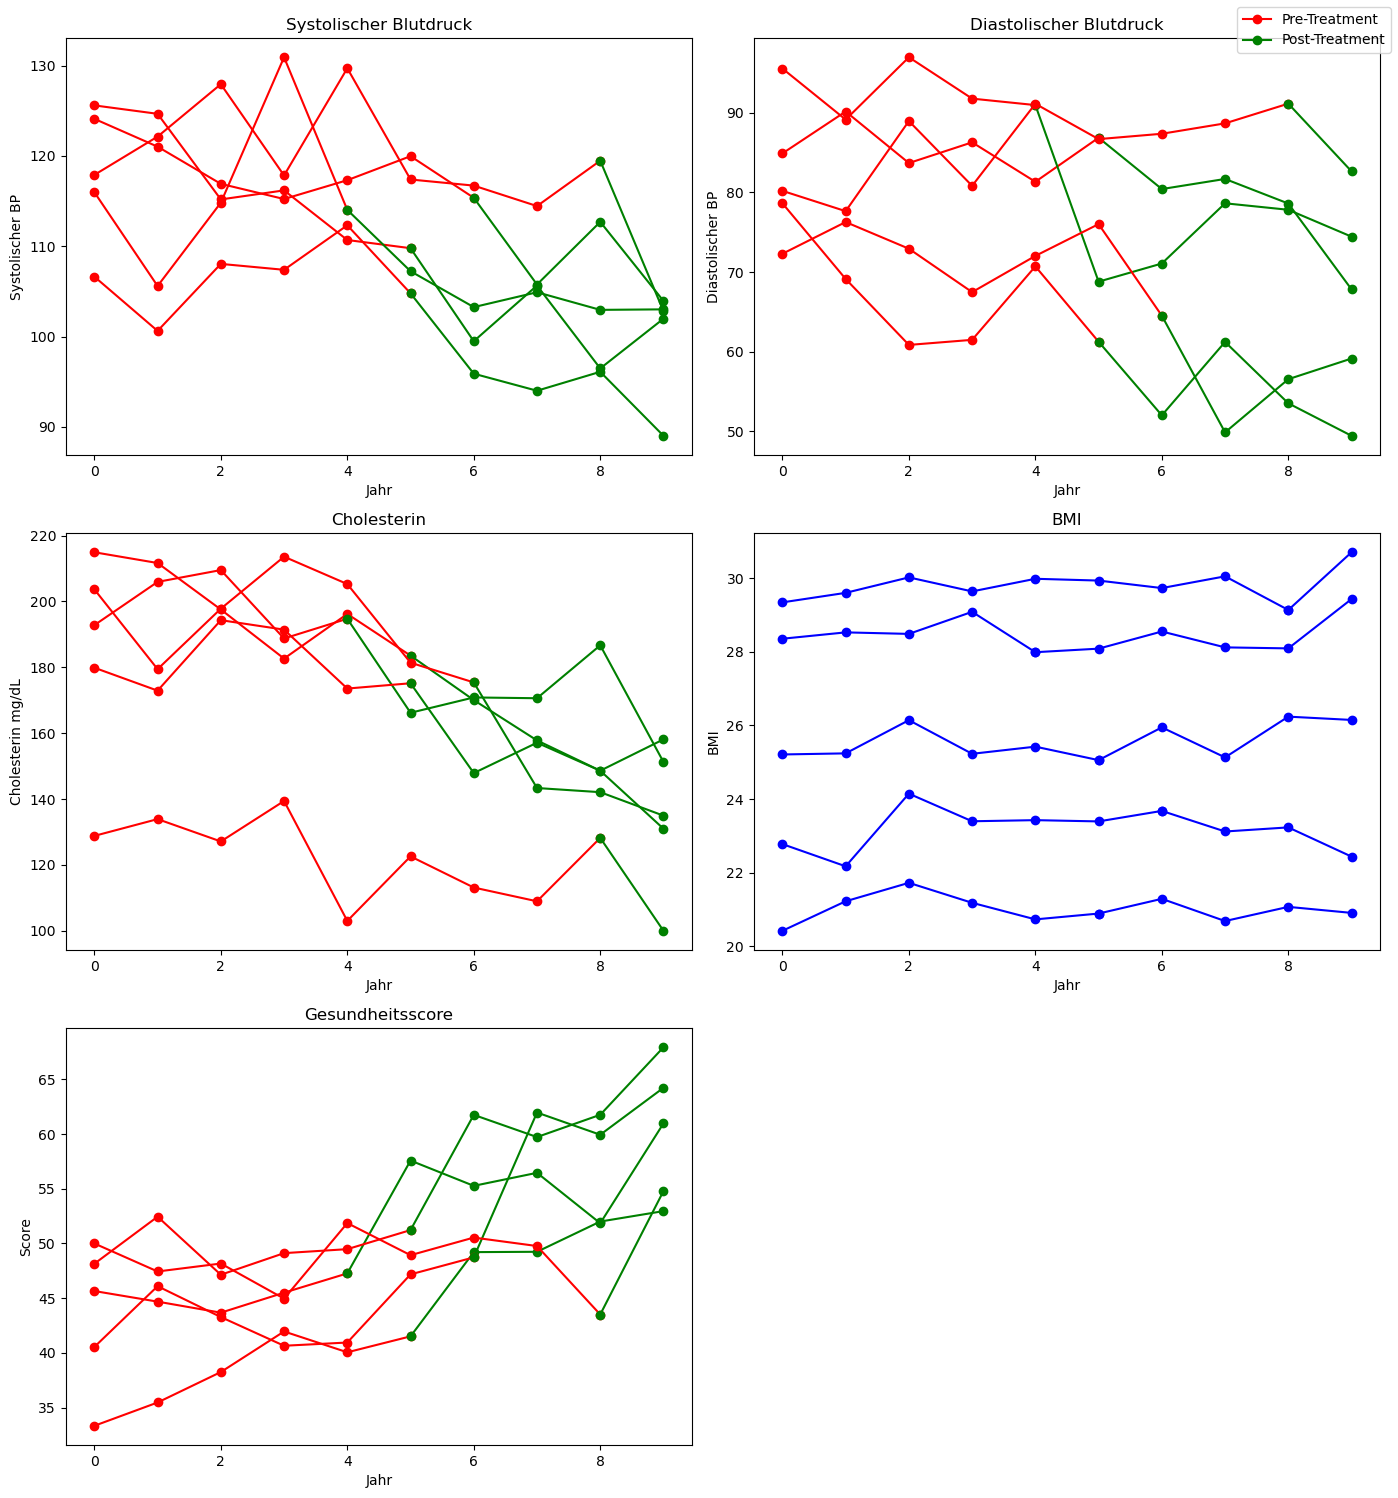
\includegraphics[width=\linewidth]{plots/Herzgesundheit_Datensatz.png}
	\caption{Simulierte Datensätze für 20 zufällig ausgewählte Patienten}
	\label{fig:sample_image}
\end{figure} 
Basierend auf diesem Simulationsdesign, welches einem Gemischten Modell folgt, können wir nun einen Likelihood-Ratio-Test durchführen. Wir trainieren dazu ein vollständiges gemischtes Modell und ein reduziertes gemischtes Modell ohne den Effekt 'Geschlecht'. Mit den log-Likelihood Werten für die trainierten Modelle führen wir den Likelihood-Ratio-Test durch. Nach 500 Wiederholungen ergibt sich ein Histogramm der Likelihood-Ratio-Test Statistik, welches, wie zu erwarten, einer $\chi^2$ Verteilung folgt. Wir wir in Abb sieht folgt das Histogramm der Test Statistik der Roten Kurve, welche die $\chi^2$ Verteilung beschreibt, ohne Verzerrung. Bis auf einzelne Ausnahmen, welche durch Instabilitäten der Berechnung immer verursacht werden können, sind die Ergebnisse immer unter der $\chi^2$ Verteilung. Dies war allerdings auch so zu erwarten, da wir ein ganz normales gemischtes Modell betrachtet hatten.
\subsection{Gemischtes Modell auf latenter Datenwolke mit separatem Training}
Nun wollen wir das gemischte Modell in einer latenten Repräsentation betrachten. Dazu wählen wir, wie schon angeführt, einen Variational-Autoencoder. Außerdem haben wir nun einen hochdimensionalen medizinischen Datensatz gegeben. Dieser ist einem echten Datensatz bestmöglich nachgebaut, allerdings kann hier aus Datenschutzgründen kein wirklich echter Datensatz benutzt werden. Wir wählen zunächst ein recht simples Encoder-Modell mit zwei Schichten und einer zweidimensionalen latenten Dimension. 
Wir trainieren zuerst den VAE separat von den gemischten Modellen. Dazu optimieren wir in der Loss-Funktion den Reconstruction Loss und die KL-Divergenz. Das vollständige und reduzierte gemischte Modell trainieren wir dann auf der latenten Datenwolke jeweils nach dem abgeschlossenen Training des VAEs. So erhalten wir wieder zwei log-likelihood Werte welche wir mit dem Likelihood-Ratio-Test auswerten können. Fassen wir alle LRT-Werte gleichermaßen wie zuvor in einem Histogramm zusammen und vergleichen mit der $\chi^2$ Verteilung, so sehen wir, dass eine bedeutende Masse dieses Mal über der $\chi^2$ Verteilung liegt. Wir sehen also, dass es zu einer Verzerrung der Inferenz kommt. 
\subsection{Gemischtes Modell auf latenter Datenwolke mit gleichzeitigem Training}
Wenn wir nun versuchen das gemischte Modell zusammen mit dem VAE in einer einzigen Loss-Funktion zu trainieren, sehen wir recht schnell, dass wir so nicht zu einem gewünschten Ergebnis kommen. Bei einem gemeinsamen Training unter der Voraussetzung, dass in der Loss-Funktion alle Parameter gleich gewichtet sind, geht die $\chi^2$ Verteilung komplett verloren. 
Fügen wir der Lossfunktion auch nur den Mean-Squarred-Error zwischen dem Encoder Output und dem Output des vollständig trainierten gemischten Modells hinzu und gewichten diesen nur minimal, so verlieren wir schon die $\chi^2$-Verteilung. Das bedeutet sobald der Encoder Einfluss auf das gemsischte Modell hat, geht die gewünschte Verteilung verloren.
Dementsprechend geht die Verteilung auch verloren, wenn wir 

%%--------------------METHODIK-----------------------------------------------
\chapter{Methodik}
\section{Vorgehen}
In den ersten Wochen habe ich mir selbst ein Simulationsdesign für einen longitudinalen medizinischen Datensatz ausgedacht und basierend darauf ein gemischtes Modell gefittet. Mit diesen simulierten Daten habe ich ein reduziertes Model mit dem vollständigen Model verglichen. Die LRT Statistik habe ich dann in einem Histogramm dargestellt.\\
\\
Wir fügen dem gemischten Modell einen festen Effekt hinzu, welcher keinen Einfluss auf die Trajektorie haben soll. In unserem Fall ist dieser feste Effekt das Geschlecht, welches keinen Einfluss auf den Verlauf einer Krankheit haben sollte.\\
\\
Mein zweites Projekt ist nun einen hoch dimensionalen medizinischen Datensatz durch den Encoder eines Variational Autoencoders im latenten Raum zu repräsentieren und dort mit einem gemischten Model darzustellen. Ähnlich wie zuvor will ich wieder eine LRT Statistik erhalten, in dem ich ein reduziertes Modell mit dem vollständigen Model vergleiche. Dazu trainiere ich in einer Schleife den Encoder und das gemischte Model für jeden Iterationsschritt neu und vergleiche die negativen Maximum Likelihood-Werte (ML-Werte) durch den Likelihood Ratio Test. Am Ende der Schleife erhalte ich wieder eine LRT Statistik, welche durch ein Histogramm dargestellt wird. Im Optimalfall ähnelt das Histogramm einer Chi-Quadrat-Verteilung mit einem Freiheitsgrad (Da das reduzierte Model nur einen festen Effekt, das Geschlecht, weniger hat).\\
\section{Experimentelles Design}
Aufbau der experimentellen Tests und Simulationen.
\section{Durchführung}
Beschreibung der durchgeführten Experimente und verwendeten Parameter.
\section{Analyse der Ergebnisse}
Diskussion der Ergebnisse im Hinblick auf die Verzerrung der Inferenz.

%%------------DISKUSSION-----------------------------------------------------
\chapter{Diskussion}
\section{Interpretation der Ergebnisse}
Tiefere Analyse der Ergebnisse und ihrer Implikationen.
\section{Vergleich mit bestehenden Arbeiten}
Wie sich die Ergebnisse zu bereits veröffentlichten Forschungen verhalten.
\section{Limitationen und Herausforderungen}
Kritische Betrachtung der Grenzen der Studie und mögliche Probleme.
\chapter{Fazit}
Zusammenfassung der wichtigsten Erkenntnisse
Praktische Implikationen: Wie die Ergebnisse in der Praxis angewendet werden können.
Empfehlungen für zukünftige Forschungen: Vorschläge für weiterführende oder ergänzende Studien.
\chapter{Anhang}
\appendix
\chapter{Appendix}
\section{Supporting Data}
\section{Some Code Listings}

\backmatter{}
\listoffigures% may be removed
\listoftables% may be removed

\nocite{Alspach:2008,GaleShapley:1962} % further literature that has not been explicitly referenced in the text
\printbibliography{} % print bibliography

\end{document}

%%% Local Variables:
%%% mode: latex
%%% TeX-engine: default
%%% TeX-command-extra-options: "-shell-escape"
%%% ispell-local-dictionary: "american"
%%% eval: (setenv "TEXINPUTS" ".//:")
%%% TeX-master: t
%%% End:
